% Graphic for TeX using PGF
% Title: /home/tobias/Documents/Studium/softwareengineering/organisation/documentations/softwareentwurf/uml-diagramms/Classdiagram-structure-engine.dia
% Creator: Dia v0.97.2
% CreationDate: Sun Oct 18 15:37:55 2015
% For: tobias
% \usepackage{tikz}
% The following commands are not supported in PSTricks at present
% We define them conditionally, so when they are implemented,
% this pgf file will use them.
\ifx\du\undefined
  \newlength{\du}
\fi
\setlength{\du}{15\unitlength}
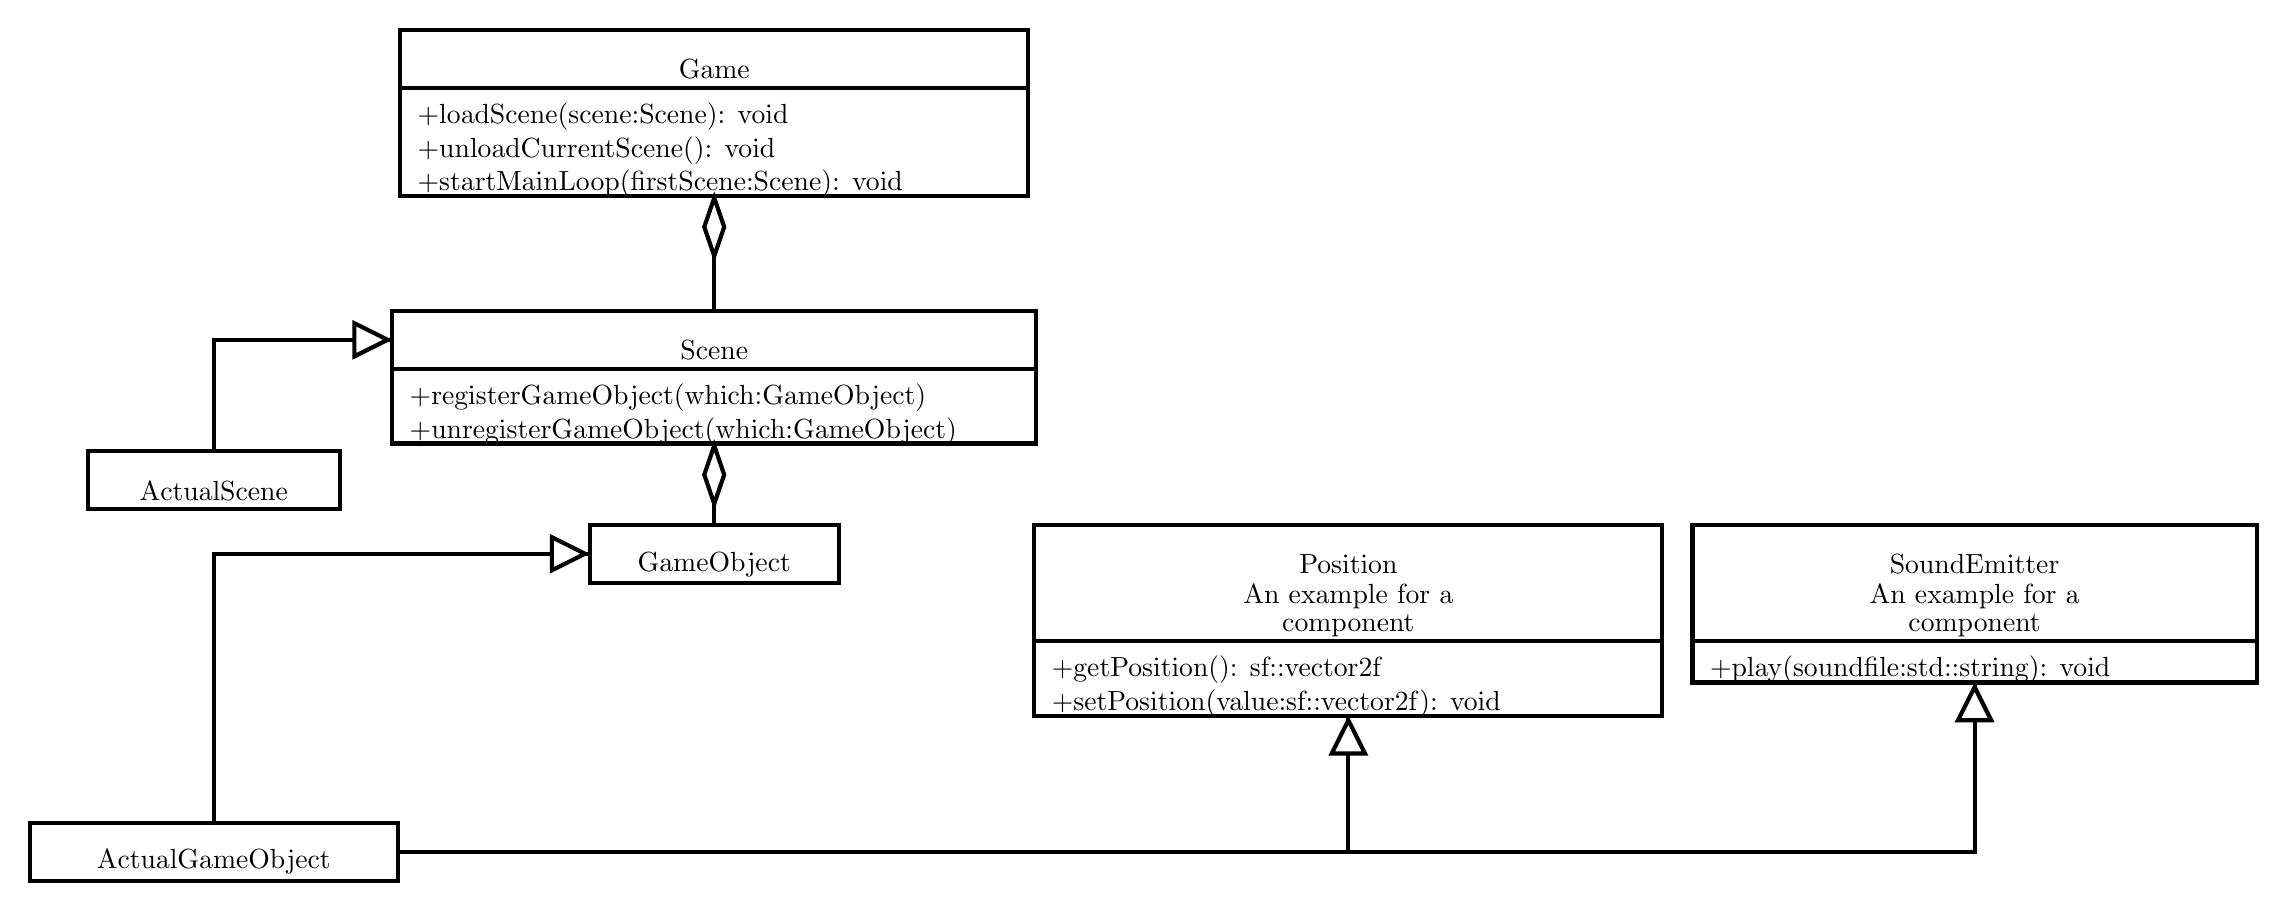
\begin{tikzpicture}
\pgftransformxscale{1.000000}
\pgftransformyscale{-1.000000}
\definecolor{dialinecolor}{rgb}{0.000000, 0.000000, 0.000000}
\pgfsetstrokecolor{dialinecolor}
\definecolor{dialinecolor}{rgb}{1.000000, 1.000000, 1.000000}
\pgfsetfillcolor{dialinecolor}
\pgfsetlinewidth{0.100000\du}
\pgfsetdash{}{0pt}
\definecolor{dialinecolor}{rgb}{1.000000, 1.000000, 1.000000}
\pgfsetfillcolor{dialinecolor}
\fill (15.424136\du,0.950000\du)--(15.424136\du,2.350000\du)--(30.554136\du,2.350000\du)--(30.554136\du,0.950000\du)--cycle;
\definecolor{dialinecolor}{rgb}{0.000000, 0.000000, 0.000000}
\pgfsetstrokecolor{dialinecolor}
\draw (15.424136\du,0.950000\du)--(15.424136\du,2.350000\du)--(30.554136\du,2.350000\du)--(30.554136\du,0.950000\du)--cycle;
% setfont left to latex
\definecolor{dialinecolor}{rgb}{0.000000, 0.000000, 0.000000}
\pgfsetstrokecolor{dialinecolor}
\node at (22.989136\du,1.900000\du){Game};
\definecolor{dialinecolor}{rgb}{1.000000, 1.000000, 1.000000}
\pgfsetfillcolor{dialinecolor}
\fill (15.424136\du,2.350000\du)--(15.424136\du,4.950000\du)--(30.554136\du,4.950000\du)--(30.554136\du,2.350000\du)--cycle;
\definecolor{dialinecolor}{rgb}{0.000000, 0.000000, 0.000000}
\pgfsetstrokecolor{dialinecolor}
\draw (15.424136\du,2.350000\du)--(15.424136\du,4.950000\du)--(30.554136\du,4.950000\du)--(30.554136\du,2.350000\du)--cycle;
% setfont left to latex
\definecolor{dialinecolor}{rgb}{0.000000, 0.000000, 0.000000}
\pgfsetstrokecolor{dialinecolor}
\node[anchor=west] at (15.574136\du,3.050000\du){+loadScene(scene:Scene): void};
% setfont left to latex
\definecolor{dialinecolor}{rgb}{0.000000, 0.000000, 0.000000}
\pgfsetstrokecolor{dialinecolor}
\node[anchor=west] at (15.574136\du,3.850000\du){+unloadCurrentScene(): void};
% setfont left to latex
\definecolor{dialinecolor}{rgb}{0.000000, 0.000000, 0.000000}
\pgfsetstrokecolor{dialinecolor}
\node[anchor=west] at (15.574136\du,4.650000\du){+startMainLoop(firstScene:Scene): void};
\pgfsetlinewidth{0.100000\du}
\pgfsetdash{}{0pt}
\definecolor{dialinecolor}{rgb}{1.000000, 1.000000, 1.000000}
\pgfsetfillcolor{dialinecolor}
\fill (15.231636\du,7.718324\du)--(15.231636\du,9.118324\du)--(30.746636\du,9.118324\du)--(30.746636\du,7.718324\du)--cycle;
\definecolor{dialinecolor}{rgb}{0.000000, 0.000000, 0.000000}
\pgfsetstrokecolor{dialinecolor}
\draw (15.231636\du,7.718324\du)--(15.231636\du,9.118324\du)--(30.746636\du,9.118324\du)--(30.746636\du,7.718324\du)--cycle;
% setfont left to latex
\definecolor{dialinecolor}{rgb}{0.000000, 0.000000, 0.000000}
\pgfsetstrokecolor{dialinecolor}
\node at (22.989136\du,8.668324\du){Scene};
\definecolor{dialinecolor}{rgb}{1.000000, 1.000000, 1.000000}
\pgfsetfillcolor{dialinecolor}
\fill (15.231636\du,9.118324\du)--(15.231636\du,10.918324\du)--(30.746636\du,10.918324\du)--(30.746636\du,9.118324\du)--cycle;
\definecolor{dialinecolor}{rgb}{0.000000, 0.000000, 0.000000}
\pgfsetstrokecolor{dialinecolor}
\draw (15.231636\du,9.118324\du)--(15.231636\du,10.918324\du)--(30.746636\du,10.918324\du)--(30.746636\du,9.118324\du)--cycle;
% setfont left to latex
\definecolor{dialinecolor}{rgb}{0.000000, 0.000000, 0.000000}
\pgfsetstrokecolor{dialinecolor}
\node[anchor=west] at (15.381636\du,9.818324\du){+registerGameObject(which:GameObject)};
% setfont left to latex
\definecolor{dialinecolor}{rgb}{0.000000, 0.000000, 0.000000}
\pgfsetstrokecolor{dialinecolor}
\node[anchor=west] at (15.381636\du,10.618324\du){+unregisterGameObject(which:GameObject)};
\pgfsetlinewidth{0.100000\du}
\pgfsetdash{}{0pt}
\definecolor{dialinecolor}{rgb}{1.000000, 1.000000, 1.000000}
\pgfsetfillcolor{dialinecolor}
\fill (19.989136\du,12.873073\du)--(19.989136\du,14.273073\du)--(25.989136\du,14.273073\du)--(25.989136\du,12.873073\du)--cycle;
\definecolor{dialinecolor}{rgb}{0.000000, 0.000000, 0.000000}
\pgfsetstrokecolor{dialinecolor}
\draw (19.989136\du,12.873073\du)--(19.989136\du,14.273073\du)--(25.989136\du,14.273073\du)--(25.989136\du,12.873073\du)--cycle;
% setfont left to latex
\definecolor{dialinecolor}{rgb}{0.000000, 0.000000, 0.000000}
\pgfsetstrokecolor{dialinecolor}
\node at (22.989136\du,13.823073\du){GameObject};
\pgfsetlinewidth{0.100000\du}
\pgfsetdash{}{0pt}
\definecolor{dialinecolor}{rgb}{1.000000, 1.000000, 1.000000}
\pgfsetfillcolor{dialinecolor}
\fill (30.700000\du,12.873073\du)--(30.700000\du,15.673073\du)--(45.830000\du,15.673073\du)--(45.830000\du,12.873073\du)--cycle;
\definecolor{dialinecolor}{rgb}{0.000000, 0.000000, 0.000000}
\pgfsetstrokecolor{dialinecolor}
\draw (30.700000\du,12.873073\du)--(30.700000\du,15.673073\du)--(45.830000\du,15.673073\du)--(45.830000\du,12.873073\du)--cycle;
% setfont left to latex
\definecolor{dialinecolor}{rgb}{0.000000, 0.000000, 0.000000}
\pgfsetstrokecolor{dialinecolor}
\node at (38.265000\du,13.823073\du){Position};
% setfont left to latex
\definecolor{dialinecolor}{rgb}{0.000000, 0.000000, 0.000000}
\pgfsetstrokecolor{dialinecolor}
\node at (38.265000\du,14.598073\du){An example for a};
\definecolor{dialinecolor}{rgb}{0.000000, 0.000000, 0.000000}
\pgfsetstrokecolor{dialinecolor}
\node at (38.265000\du,15.298073\du){component};
\definecolor{dialinecolor}{rgb}{1.000000, 1.000000, 1.000000}
\pgfsetfillcolor{dialinecolor}
\fill (30.700000\du,15.673073\du)--(30.700000\du,17.473073\du)--(45.830000\du,17.473073\du)--(45.830000\du,15.673073\du)--cycle;
\definecolor{dialinecolor}{rgb}{0.000000, 0.000000, 0.000000}
\pgfsetstrokecolor{dialinecolor}
\draw (30.700000\du,15.673073\du)--(30.700000\du,17.473073\du)--(45.830000\du,17.473073\du)--(45.830000\du,15.673073\du)--cycle;
% setfont left to latex
\definecolor{dialinecolor}{rgb}{0.000000, 0.000000, 0.000000}
\pgfsetstrokecolor{dialinecolor}
\node[anchor=west] at (30.850000\du,16.373073\du){+getPosition(): sf::vector2f};
% setfont left to latex
\definecolor{dialinecolor}{rgb}{0.000000, 0.000000, 0.000000}
\pgfsetstrokecolor{dialinecolor}
\node[anchor=west] at (30.850000\du,17.173073\du){+setPosition(value:sf::vector2f): void};
\pgfsetlinewidth{0.100000\du}
\pgfsetdash{}{0pt}
\definecolor{dialinecolor}{rgb}{1.000000, 1.000000, 1.000000}
\pgfsetfillcolor{dialinecolor}
\fill (46.555950\du,12.873073\du)--(46.555950\du,15.673073\du)--(60.145950\du,15.673073\du)--(60.145950\du,12.873073\du)--cycle;
\definecolor{dialinecolor}{rgb}{0.000000, 0.000000, 0.000000}
\pgfsetstrokecolor{dialinecolor}
\draw (46.555950\du,12.873073\du)--(46.555950\du,15.673073\du)--(60.145950\du,15.673073\du)--(60.145950\du,12.873073\du)--cycle;
% setfont left to latex
\definecolor{dialinecolor}{rgb}{0.000000, 0.000000, 0.000000}
\pgfsetstrokecolor{dialinecolor}
\node at (53.350950\du,13.823073\du){SoundEmitter};
% setfont left to latex
\definecolor{dialinecolor}{rgb}{0.000000, 0.000000, 0.000000}
\pgfsetstrokecolor{dialinecolor}
\node at (53.350950\du,14.598073\du){An example for a};
\definecolor{dialinecolor}{rgb}{0.000000, 0.000000, 0.000000}
\pgfsetstrokecolor{dialinecolor}
\node at (53.350950\du,15.298073\du){component};
\definecolor{dialinecolor}{rgb}{1.000000, 1.000000, 1.000000}
\pgfsetfillcolor{dialinecolor}
\fill (46.555950\du,15.673073\du)--(46.555950\du,16.673073\du)--(60.145950\du,16.673073\du)--(60.145950\du,15.673073\du)--cycle;
\definecolor{dialinecolor}{rgb}{0.000000, 0.000000, 0.000000}
\pgfsetstrokecolor{dialinecolor}
\draw (46.555950\du,15.673073\du)--(46.555950\du,16.673073\du)--(60.145950\du,16.673073\du)--(60.145950\du,15.673073\du)--cycle;
% setfont left to latex
\definecolor{dialinecolor}{rgb}{0.000000, 0.000000, 0.000000}
\pgfsetstrokecolor{dialinecolor}
\node[anchor=west] at (46.705950\du,16.373073\du){+play(soundfile:std::string): void};
\pgfsetlinewidth{0.100000\du}
\pgfsetdash{}{0pt}
\definecolor{dialinecolor}{rgb}{1.000000, 1.000000, 1.000000}
\pgfsetfillcolor{dialinecolor}
\fill (6.500000\du,20.050000\du)--(6.500000\du,21.450000\du)--(15.362500\du,21.450000\du)--(15.362500\du,20.050000\du)--cycle;
\definecolor{dialinecolor}{rgb}{0.000000, 0.000000, 0.000000}
\pgfsetstrokecolor{dialinecolor}
\draw (6.500000\du,20.050000\du)--(6.500000\du,21.450000\du)--(15.362500\du,21.450000\du)--(15.362500\du,20.050000\du)--cycle;
% setfont left to latex
\definecolor{dialinecolor}{rgb}{0.000000, 0.000000, 0.000000}
\pgfsetstrokecolor{dialinecolor}
\node at (10.931250\du,21.000000\du){ActualGameObject};
\pgfsetlinewidth{0.100000\du}
\pgfsetdash{}{0pt}
\pgfsetmiterjoin
\pgfsetbuttcap
{
\definecolor{dialinecolor}{rgb}{0.000000, 0.000000, 0.000000}
\pgfsetfillcolor{dialinecolor}
% was here!!!
\definecolor{dialinecolor}{rgb}{0.000000, 0.000000, 0.000000}
\pgfsetstrokecolor{dialinecolor}
\draw (19.989136\du,13.573073\du)--(10.931250\du,13.573073\du)--(10.931250\du,20.050000\du);
}
\definecolor{dialinecolor}{rgb}{0.000000, 0.000000, 0.000000}
\pgfsetstrokecolor{dialinecolor}
\draw (19.077333\du,13.573073\du)--(10.931250\du,13.573073\du)--(10.931250\du,20.050000\du);
\pgfsetmiterjoin
\definecolor{dialinecolor}{rgb}{1.000000, 1.000000, 1.000000}
\pgfsetfillcolor{dialinecolor}
\fill (19.077333\du,13.973073\du)--(19.877333\du,13.573073\du)--(19.077333\du,13.173073\du)--cycle;
\pgfsetlinewidth{0.100000\du}
\pgfsetdash{}{0pt}
\pgfsetmiterjoin
\definecolor{dialinecolor}{rgb}{0.000000, 0.000000, 0.000000}
\pgfsetstrokecolor{dialinecolor}
\draw (19.077333\du,13.973073\du)--(19.877333\du,13.573073\du)--(19.077333\du,13.173073\du)--cycle;
% setfont left to latex
\pgfsetlinewidth{0.100000\du}
\pgfsetdash{}{0pt}
\pgfsetmiterjoin
\pgfsetbuttcap
{
\definecolor{dialinecolor}{rgb}{0.000000, 0.000000, 0.000000}
\pgfsetfillcolor{dialinecolor}
% was here!!!
\definecolor{dialinecolor}{rgb}{0.000000, 0.000000, 0.000000}
\pgfsetstrokecolor{dialinecolor}
\draw (38.265000\du,17.473073\du)--(38.265000\du,20.750000\du)--(15.362500\du,20.750000\du);
}
\definecolor{dialinecolor}{rgb}{0.000000, 0.000000, 0.000000}
\pgfsetstrokecolor{dialinecolor}
\draw (38.265000\du,18.384876\du)--(38.265000\du,20.750000\du)--(15.362500\du,20.750000\du);
\pgfsetmiterjoin
\definecolor{dialinecolor}{rgb}{1.000000, 1.000000, 1.000000}
\pgfsetfillcolor{dialinecolor}
\fill (38.665000\du,18.384876\du)--(38.265000\du,17.584876\du)--(37.865000\du,18.384876\du)--cycle;
\pgfsetlinewidth{0.100000\du}
\pgfsetdash{}{0pt}
\pgfsetmiterjoin
\definecolor{dialinecolor}{rgb}{0.000000, 0.000000, 0.000000}
\pgfsetstrokecolor{dialinecolor}
\draw (38.665000\du,18.384876\du)--(38.265000\du,17.584876\du)--(37.865000\du,18.384876\du)--cycle;
% setfont left to latex
\pgfsetlinewidth{0.100000\du}
\pgfsetdash{}{0pt}
\pgfsetmiterjoin
\pgfsetbuttcap
{
\definecolor{dialinecolor}{rgb}{0.000000, 0.000000, 0.000000}
\pgfsetfillcolor{dialinecolor}
% was here!!!
\definecolor{dialinecolor}{rgb}{0.000000, 0.000000, 0.000000}
\pgfsetstrokecolor{dialinecolor}
\draw (53.350950\du,16.673073\du)--(53.350950\du,20.750000\du)--(15.362500\du,20.750000\du);
}
\definecolor{dialinecolor}{rgb}{0.000000, 0.000000, 0.000000}
\pgfsetstrokecolor{dialinecolor}
\draw (53.350950\du,17.584876\du)--(53.350950\du,20.750000\du)--(15.362500\du,20.750000\du);
\pgfsetmiterjoin
\definecolor{dialinecolor}{rgb}{1.000000, 1.000000, 1.000000}
\pgfsetfillcolor{dialinecolor}
\fill (53.750950\du,17.584876\du)--(53.350950\du,16.784876\du)--(52.950950\du,17.584876\du)--cycle;
\pgfsetlinewidth{0.100000\du}
\pgfsetdash{}{0pt}
\pgfsetmiterjoin
\definecolor{dialinecolor}{rgb}{0.000000, 0.000000, 0.000000}
\pgfsetstrokecolor{dialinecolor}
\draw (53.750950\du,17.584876\du)--(53.350950\du,16.784876\du)--(52.950950\du,17.584876\du)--cycle;
% setfont left to latex
\pgfsetlinewidth{0.100000\du}
\pgfsetdash{}{0pt}
\definecolor{dialinecolor}{rgb}{1.000000, 1.000000, 1.000000}
\pgfsetfillcolor{dialinecolor}
\fill (7.897500\du,11.100000\du)--(7.897500\du,12.500000\du)--(13.965000\du,12.500000\du)--(13.965000\du,11.100000\du)--cycle;
\definecolor{dialinecolor}{rgb}{0.000000, 0.000000, 0.000000}
\pgfsetstrokecolor{dialinecolor}
\draw (7.897500\du,11.100000\du)--(7.897500\du,12.500000\du)--(13.965000\du,12.500000\du)--(13.965000\du,11.100000\du)--cycle;
% setfont left to latex
\definecolor{dialinecolor}{rgb}{0.000000, 0.000000, 0.000000}
\pgfsetstrokecolor{dialinecolor}
\node at (10.931250\du,12.050000\du){ActualScene};
\pgfsetlinewidth{0.100000\du}
\pgfsetdash{}{0pt}
\pgfsetmiterjoin
\pgfsetbuttcap
{
\definecolor{dialinecolor}{rgb}{0.000000, 0.000000, 0.000000}
\pgfsetfillcolor{dialinecolor}
% was here!!!
\definecolor{dialinecolor}{rgb}{0.000000, 0.000000, 0.000000}
\pgfsetstrokecolor{dialinecolor}
\draw (15.231636\du,8.418324\du)--(10.931250\du,8.418324\du)--(10.931250\du,11.100000\du);
}
\definecolor{dialinecolor}{rgb}{0.000000, 0.000000, 0.000000}
\pgfsetstrokecolor{dialinecolor}
\draw (14.319833\du,8.418324\du)--(10.931250\du,8.418324\du)--(10.931250\du,11.100000\du);
\pgfsetmiterjoin
\definecolor{dialinecolor}{rgb}{1.000000, 1.000000, 1.000000}
\pgfsetfillcolor{dialinecolor}
\fill (14.319833\du,8.818324\du)--(15.119833\du,8.418324\du)--(14.319833\du,8.018324\du)--cycle;
\pgfsetlinewidth{0.100000\du}
\pgfsetdash{}{0pt}
\pgfsetmiterjoin
\definecolor{dialinecolor}{rgb}{0.000000, 0.000000, 0.000000}
\pgfsetstrokecolor{dialinecolor}
\draw (14.319833\du,8.818324\du)--(15.119833\du,8.418324\du)--(14.319833\du,8.018324\du)--cycle;
% setfont left to latex
\pgfsetlinewidth{0.100000\du}
\pgfsetdash{}{0pt}
\pgfsetmiterjoin
\pgfsetbuttcap
{
\definecolor{dialinecolor}{rgb}{0.000000, 0.000000, 0.000000}
\pgfsetfillcolor{dialinecolor}
% was here!!!
\definecolor{dialinecolor}{rgb}{0.000000, 0.000000, 0.000000}
\pgfsetstrokecolor{dialinecolor}
\draw (22.989136\du,5.000250\du)--(22.989136\du,5.750250\du)--(22.989136\du,7.617921\du)--(22.989136\du,7.667921\du);
}
\definecolor{dialinecolor}{rgb}{0.000000, 0.000000, 0.000000}
\pgfsetstrokecolor{dialinecolor}
\draw (22.989136\du,6.258829\du)--(22.989136\du,5.750250\du)--(22.989136\du,7.617921\du)--(22.989136\du,7.667921\du);
\pgfsetdash{}{0pt}
\pgfsetmiterjoin
\pgfsetbuttcap
\definecolor{dialinecolor}{rgb}{1.000000, 1.000000, 1.000000}
\pgfsetfillcolor{dialinecolor}
\fill (22.989136\du,5.000250\du)--(23.229136\du,5.700250\du)--(22.989136\du,6.400250\du)--(22.749136\du,5.700250\du)--cycle;
\pgfsetlinewidth{0.100000\du}
\pgfsetdash{}{0pt}
\pgfsetmiterjoin
\pgfsetbuttcap
\definecolor{dialinecolor}{rgb}{0.000000, 0.000000, 0.000000}
\pgfsetstrokecolor{dialinecolor}
\draw (22.989136\du,5.000250\du)--(23.229136\du,5.700250\du)--(22.989136\du,6.400250\du)--(22.749136\du,5.700250\du)--cycle;
% setfont left to latex
\pgfsetlinewidth{0.100000\du}
\pgfsetdash{}{0pt}
\pgfsetmiterjoin
\pgfsetbuttcap
{
\definecolor{dialinecolor}{rgb}{0.000000, 0.000000, 0.000000}
\pgfsetfillcolor{dialinecolor}
% was here!!!
\definecolor{dialinecolor}{rgb}{0.000000, 0.000000, 0.000000}
\pgfsetstrokecolor{dialinecolor}
\draw (22.989136\du,10.968727\du)--(22.989136\du,11.718727\du)--(22.989136\du,12.772707\du)--(22.989136\du,12.822707\du);
}
\definecolor{dialinecolor}{rgb}{0.000000, 0.000000, 0.000000}
\pgfsetstrokecolor{dialinecolor}
\draw (22.989136\du,12.227306\du)--(22.989136\du,11.718727\du)--(22.989136\du,12.772707\du)--(22.989136\du,12.822707\du);
\pgfsetdash{}{0pt}
\pgfsetmiterjoin
\pgfsetbuttcap
\definecolor{dialinecolor}{rgb}{1.000000, 1.000000, 1.000000}
\pgfsetfillcolor{dialinecolor}
\fill (22.989136\du,10.968727\du)--(23.229136\du,11.668727\du)--(22.989136\du,12.368727\du)--(22.749136\du,11.668727\du)--cycle;
\pgfsetlinewidth{0.100000\du}
\pgfsetdash{}{0pt}
\pgfsetmiterjoin
\pgfsetbuttcap
\definecolor{dialinecolor}{rgb}{0.000000, 0.000000, 0.000000}
\pgfsetstrokecolor{dialinecolor}
\draw (22.989136\du,10.968727\du)--(23.229136\du,11.668727\du)--(22.989136\du,12.368727\du)--(22.749136\du,11.668727\du)--cycle;
% setfont left to latex
\end{tikzpicture}
